\documentclass[border=3pt]{standalone}
% Shared preamble for every generated figure.
% Matches the report: newtx (Times), greyscale, square boxes.
\usepackage{newtxtext,newtxmath}
% newtx's typewriter (txtt) draws a slashed zero; use Latin Modern instead.
\renewcommand{\ttdefault}{lmtt}
\usepackage{tikz}
\usetikzlibrary{positioning,arrows.meta,calc,fit,backgrounds,shapes.geometric,
                decorations.pathreplacing,decorations.pathmorphing,matrix,patterns}

\definecolor{figgrey}{gray}{0.88}
\definecolor{figmid}{gray}{0.60}
\definecolor{figdark}{gray}{0.35}

\tikzset{
  fig/.style={font=\small},
  box/.style={draw,thick,minimum height=8mm,minimum width=22mm,align=center,
              inner sep=2pt,font=\small},
  greybox/.style={box,fill=figgrey},
  smallbox/.style={draw,minimum height=6mm,minimum width=16mm,align=center,
                   inner sep=2pt,font=\scriptsize},
  ln/.style={-{Stealth[length=2.2mm,width=1.8mm]},thick},
  lnb/.style={{Stealth[length=2.2mm,width=1.8mm]}-{Stealth[length=2.2mm,width=1.8mm]},thick},
  lbl/.style={font=\scriptsize,inner sep=1.5pt},
  note/.style={font=\scriptsize\itshape,inner sep=1.5pt},
}

\begin{document}
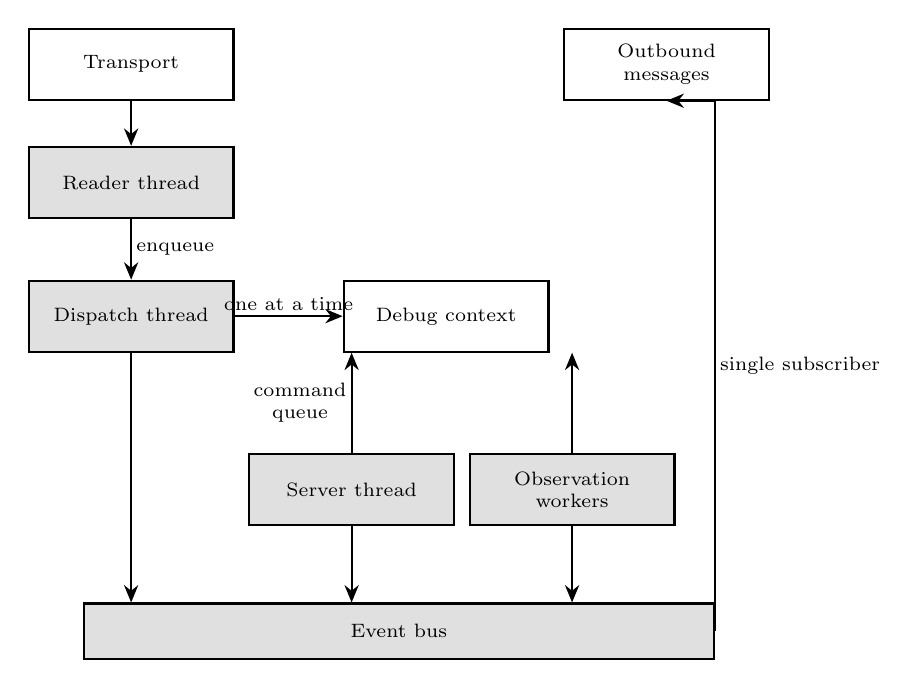
\begin{tikzpicture}[fig,
  th/.style={draw,thick,minimum height=9mm,minimum width=26mm,align=center,
             font=\scriptsize,fill=figgrey},
  res/.style={draw,thick,minimum height=9mm,minimum width=26mm,align=center,
              font=\scriptsize},
  bus/.style={draw,thick,minimum height=7mm,minimum width=80mm,align=center,
              font=\scriptsize,fill=figgrey}]

% Row 0: Transport and Outbound
\node[res] (tr) at (0,0) {Transport};
\node[res] (out) at (68mm,0) {Outbound\\messages};

% Row 1: Reader thread
\node[th] (rt) at (0,-15mm) {Reader thread};
\draw[ln] (tr) -- (rt);

% Row 2: Dispatch thread and Debug context
\node[th] (dt) at (0,-32mm) {Dispatch thread};
\node[res] (dc) at (40mm,-32mm) {Debug context};
\draw[ln] (rt) -- node[lbl,right]{enqueue} (dt);
\draw[ln] (dt) -- node[lbl,above]{one at a time} (dc);

% Row 3: Server thread and Observation workers, under debug context
\node[th] (st) at (28mm,-54mm) {Server thread};
\node[th] (ow) at (56mm,-54mm) {Observation\\workers};
\draw[ln] (st.north) -- node[lbl,left,align=center]{command\\queue} (st.north |- dc.south);
\draw[ln] (ow.north) -- (ow.north |- dc.south);

% Row 4: Event bus
\node[bus] (eb) at (34mm,-72mm) {Event bus};

% Producers to event bus
\draw[ln] (dt.south) -- (dt.south |- eb.north);
\draw[ln] (st.south) -- (st.south |- eb.north);
\draw[ln] (ow.south) -- (ow.south |- eb.north);

% Event bus to outbound messages
\draw[ln] (eb.east) -- ++(0mm,0) |- node[lbl,right,pos=0.25]{single subscriber} (out.south);

\end{tikzpicture}
\end{document}
